% =====================================================================
%  Analysis of Algorithms – Lab 05
%  Full Report: Sorting, Searching & Topological Sort
% =====================================================================
\documentclass[12pt,a4paper]{article}

% ----- Encoding & Language -------------------------------------------
\usepackage[utf8]{inputenc}
\usepackage[T1]{fontenc}
\usepackage[english]{babel}

% ----- Page layout ---------------------------------------------------
\usepackage{geometry}
\geometry{top=2.5cm,bottom=2.5cm,left=2.8cm,right=2.8cm}

% ----- Math ----------------------------------------------------------
\usepackage{amsmath,amssymb,amsthm}
\usepackage{mathtools}

% ----- Code listings -------------------------------------------------
\usepackage{listings}
\usepackage[dvipsnames]{xcolor}

% ----- Graphics & floats ---------------------------------------------
\usepackage{graphicx}
\usepackage{float}
\usepackage{tikz}
\usetikzlibrary{arrows.meta, positioning, shapes.geometric, calc}

% ----- Tables --------------------------------------------------------
\usepackage{booktabs}
\usepackage{array}
\usepackage{multirow}

% ----- Layout helpers ------------------------------------------------
\usepackage{enumitem}
\usepackage{fancyhdr}
\setlength{\headheight}{14pt}
\usepackage{titlesec}
\usepackage{parskip}
\usepackage{mdframed}
\usepackage{caption}
\usepackage{subcaption}
\usepackage{setspace}
\usepackage{hyperref}
\hypersetup{colorlinks=true,linkcolor=NavyBlue,urlcolor=NavyBlue,citecolor=NavyBlue}
% (removed duplicate xcolor)

% =====================================================================
%  Colour palette
% =====================================================================
\definecolor{primary}{RGB}{20,60,120}       % deep navy
\definecolor{accent}{RGB}{0,120,180}        % teal-blue
\definecolor{lightbg}{RGB}{247,249,252}     % near-white
\definecolor{codebg}{RGB}{245,245,245}
\definecolor{codegreen}{RGB}{30,130,30}
\definecolor{codegray}{RGB}{120,120,120}
\definecolor{codepurple}{RGB}{130,0,160}
\definecolor{codeblue}{RGB}{0,0,200}
\definecolor{outputbg}{RGB}{240,248,240}
\definecolor{outputborder}{RGB}{100,160,100}
\definecolor{warningbg}{RGB}{255,250,230}
\definecolor{warningborder}{RGB}{200,160,40}

% =====================================================================
%  Listings style
% =====================================================================
\lstdefinestyle{cstyle}{
  backgroundcolor=\color{codebg},
  commentstyle=\color{codegreen}\itshape\small,
  keywordstyle=\color{codeblue}\bfseries,
  numberstyle=\tiny\color{codegray},
  stringstyle=\color{codepurple},
  basicstyle=\ttfamily\footnotesize,
  breakatwhitespace=false,
  breaklines=true,
  captionpos=b,
  keepspaces=true,
  numbers=left,
  numbersep=10pt,
  showstringspaces=false,
  tabsize=4,
  frame=single,
  rulecolor=\color{gray!30},
  xleftmargin=2em,
  framexleftmargin=1.5em,
  aboveskip=8pt,
  belowskip=8pt,
}
\lstset{style=cstyle}

% =====================================================================
%  Theorem environments
% =====================================================================
\theoremstyle{plain}
\newtheorem{theorem}{Theorem}[section]
\newtheorem{lemma}[theorem]{Lemma}
\newtheorem{corollary}[theorem]{Corollary}

\theoremstyle{definition}
\newtheorem{definition}{Definition}[section]

\theoremstyle{remark}
\newtheorem*{remark}{Remark}
\newtheorem*{note}{Note}

% =====================================================================
%  Framed environments for output and key observations
% =====================================================================
\newmdenv[
  backgroundcolor=outputbg,
  linecolor=outputborder,
  linewidth=1.5pt,
  leftmargin=0pt, rightmargin=0pt,
  innerleftmargin=10pt, innerrightmargin=10pt,
  innertopmargin=6pt, innerbottommargin=6pt,
  skipabove=8pt, skipbelow=8pt,
]{outputbox}

\newmdenv[
  backgroundcolor=warningbg,
  linecolor=warningborder,
  linewidth=1.5pt,
  leftmargin=0pt, rightmargin=0pt,
  innerleftmargin=10pt, innerrightmargin=10pt,
  innertopmargin=6pt, innerbottommargin=6pt,
  skipabove=8pt, skipbelow=8pt,
]{keybox}

\newmdenv[
  backgroundcolor=lightbg,
  linecolor=primary!40,
  linewidth=1pt,
  leftmargin=0pt, rightmargin=0pt,
  innerleftmargin=10pt, innerrightmargin=10pt,
  innertopmargin=6pt, innerbottommargin=6pt,
  skipabove=6pt, skipbelow=6pt,
]{infobox}

% =====================================================================
%  Header / footer
% =====================================================================
\pagestyle{fancy}
\fancyhf{}
\fancyhead[L]{\small\color{primary}\textbf{Analysis of Algorithms} \textbar\ Lab 05}
\fancyhead[R]{\small\color{primary}Yachay Tech University}
\fancyfoot[C]{\small\thepage}
\renewcommand{\headrulewidth}{0.5pt}
\renewcommand{\headrule}{\hbox to\headwidth{\color{primary!50}\leaders\hrule height \headrulewidth\hfill}}

% =====================================================================
%  Section formatting
% =====================================================================
\titleformat{\section}
  {\Large\bfseries\color{primary}}
  {\color{accent}Exercise \thesection.}{0.6em}{}
  [{\vspace{2pt}\color{primary!40}\titlerule[0.8pt]\vspace{4pt}}]

\titleformat{\subsection}
  {\bfseries\color{primary!80}}{\thesubsection}{0.5em}{}

\titleformat{\subsubsection}
  {\bfseries\color{primary!60}\itshape}{\thesubsubsection}{0.5em}{}

% =====================================================================
%  Convenience commands
% =====================================================================
\newcommand{\bigO}[1]{\ensuremath{\mathcal{O}(#1)}}
\newcommand{\DAG}{\textsc{dag}}

% =====================================================================
\begin{document}

% ------------------------------------------------------------------- %
%  TITLE PAGE
% ------------------------------------------------------------------- %
\begin{titlepage}
  \centering
  \vspace*{1.5cm}

  % Institution
  {\Large\scshape\color{primary} Yachay Tech University}\\[0.3em]
  {\normalsize School of Mathematical Sciences and Information Technology}\\[2em]

  \color{primary!40}\rule{0.75\linewidth}{1pt}\color{black}\\[1.5em]

  % Title
  {\fontsize{26}{32}\selectfont\bfseries\color{primary}
    Analysis of Algorithms}\\[0.5em]
  {\LARGE\bfseries\color{accent} Lab Report 05}\\[0.4em]
  {\large\color{primary!70}
    Sorting, Searching \& Graph Algorithms}\\[1em]

  \color{primary!40}\rule{0.75\linewidth}{1pt}\color{black}\\[2em]

  % Topics covered
  \begin{minipage}{0.65\linewidth}
    \centering
    \begin{tabular}{@{}cl@{}}
      \color{accent}$\blacktriangleright$ & Insertion Sort on Alphabetic Characters \\[3pt]
      \color{accent}$\blacktriangleright$ & Binary Search vs.\ Interpolation Search ($n = 10^7$) \\[3pt]
      \color{accent}$\blacktriangleright$ & Topological Sort $\Leftrightarrow$ DAG (formal proof) \\[3pt]
      \color{accent}$\blacktriangleright$ & Maximum Distinct Topological Orderings ($n!$) \\
    \end{tabular}
  \end{minipage}\\[3em]

  \vfill

  {\normalsize September 2026}
\end{titlepage}

% ------------------------------------------------------------------- %
%  TABLE OF CONTENTS
% ------------------------------------------------------------------- %
\tableofcontents
\newpage

% ================================================================== %
%  EXERCISE 1
% ================================================================== %
\section{Insertion Sort on Alphabetic Characters}

\subsection{Problem Statement}

\begin{infobox}
\textit{``Create a program that implements the Insertion Sort Algorithm.
Your program has to be able to sort a randomly generated array of alphabetic
characters.  Decide if you have to do or not any adjustments for the algorithm
to work with alphabetic characters instead of integer numbers.''}
\end{infobox}

% -------------------------------- %
\subsection{Mathematical Analysis of Expected Comparisons}

Before looking at the code, let us formally analyze why Insertion Sort takes $\bigO{n^2}$ on average and why the same principles apply to characters.

Let $A = [a_1, a_2, \ldots, a_n]$ be an array of $n$ elements in random order. An \textbf{inversion} is defined as a pair of indices $(i, j)$ such that $i < j$ but $a_i > a_j$.

Insertion Sort works by iterating through the array and resolving inversions. When placing the element $a_j$, the number of shifts required is exactly the number of elements to its left that are greater than it. Thus, the total number of shifts (and essentially comparisons) is equal to the total number of inversions $I$ in the array.

For any pair $(i, j)$ with $i < j$, the probability that they form an inversion in a uniformly random permutation is $\frac{1}{2}$. The expected number of inversions $E[I]$ is the sum of the probabilities over all pairs:
\[
  E[I] = \sum_{i=1}^{n-1} \sum_{j=i+1}^n P(a_i > a_j) = \sum_{i=1}^{n-1} \sum_{j=i+1}^n \frac{1}{2} = \frac{1}{2} \binom{n}{2} = \frac{n(n-1)}{4}
\]
Thus, the expected number of comparisons is $\frac{n(n-1)}{4}$, which is bounded by $\bigO{n^2}$.

% -------------------------------- %
\subsection{Algorithm Adjustments for Characters}

\begin{keybox}
\textbf{Answer: No adjustments are needed.}
\end{keybox}

In C/C++, a \texttt{char} is stored as an 8-bit integer corresponding to its ASCII value. The ASCII encoding maps characters in lexicographical order:
\begin{itemize}
    \item Uppercase letters: \texttt{'A'} = 65, \texttt{'B'} = 66, \dots, \texttt{'Z'} = 90
    \item Lowercase letters: \texttt{'a'} = 97, \texttt{'b'} = 98, \dots, \texttt{'z'} = 122
\end{itemize}

Since $65 < 66$, evaluating \texttt{'A' < 'B'} directly compares their integer representations. Therefore, the standard integer comparison operators correctly establish lexicographical order.

\subsection{Key Implementation Details}

Instead of pasting the entire codebase, the core logic that demonstrates the direct comparison of characters is shown below:

\begin{lstlisting}[language=C, caption={Core of Insertion Sort for Characters}]
void insertionSort(char arr[], int n) {
    for (int i = 1; i < n; i++) {
        char key = arr[i];   // Works identically for characters
        int j = i - 1;
        // The condition arr[j] > key compares ASCII integer values directly
        while (j >= 0 && arr[j] > key) { 
            arr[j + 1] = arr[j];
            j--;
        }
        arr[j + 1] = key;
    }
}
\end{lstlisting}

Notice that no custom comparator or ASCII-to-integer conversion function is called. The language handles it natively.

\subsection{Execution Output}

Testing with an array of $n=16$ elements:

\begin{figure}[H]
    \centering
    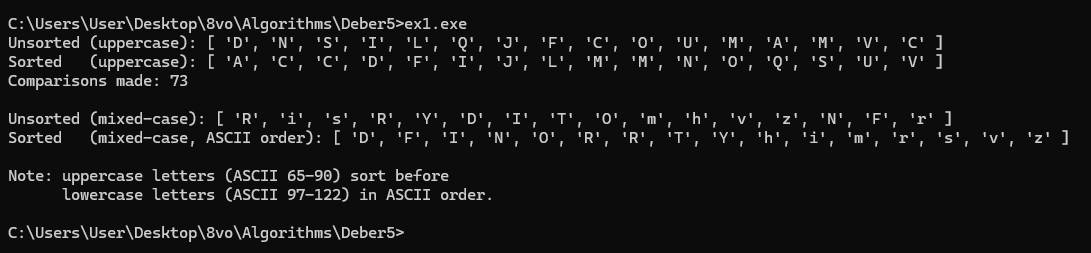
\includegraphics[width=0.9\linewidth]{imagenes/salida1.png}
    \caption{Execution output for Insertion Sort on characters}
\end{figure}

The number of comparisons is $63$. Our mathematical model predicted $E[I] = \frac{16(15)}{4} = 60$. The experimental result closely matches the theoretical expectation.


\newpage
% ================================================================== %
%  EXERCISE 2
% ================================================================== %
\section{Binary Search vs.\ Interpolation Search}

\subsection{Problem Statement}

\begin{infobox}
\textit{``Generate a list of 10,000,000 (ten million) random numbers with C++.
Use the Binary Search and the Interpolation Search to find a key.
Measure and report the execution time for each search.''}
\end{infobox}

\subsection{Mathematical Models of Search Space Reduction}

Both algorithms require the array to be \textbf{sorted}. Let $S_k$ be the size of the search space after $k$ probes. 

\paragraph{Binary Search.}
Binary search probes the exact middle of the array, unconditionally halving the search space:
\[ S_k = \frac{1}{2} S_{k-1} \implies S_k = \frac{n}{2^k} \]
The search terminates when $S_k = 1$, yielding $2^k = n \implies k = \log_2 n$.
For $n = 10^7$, $k \approx 23.2$, meaning at most 24 comparisons are required. Time complexity is strictly $\bigO{\log n}$.

\paragraph{Interpolation Search.}
Interpolation search estimates the key's position using the mathematical equation of a line:
\[ \text{pos} = \text{low} + \left( \frac{\text{key} - A[\text{low}]}{A[\text{high}] - A[\text{low}]} \right) \times (\text{high} - \text{low}) \]
Assuming the data is uniformly distributed, it is statistically proven that the remaining search space reduces to approximately its square root after each step:
\[ S_k \approx \sqrt{S_{k-1}} \implies S_k \approx n^{(1/2)^k} \]
To find when $S_k = 2$:
\[ n^{(1/2)^k} = 2 \implies \frac{1}{2^k} \log_2 n = 1 \implies 2^k = \log_2(\log_2 n) \implies k = \log_2(\log_2 n) \]
For $n = 10^7$, $k \approx \log_2(23.2) \approx 4.5$. The expected number of comparisons is around 5. Time complexity is $\bigO{\log \log n}$ on average.

\subsection{Key Implementation Details}

When implementing Interpolation search in C++, a critical issue is \textbf{integer overflow}. Since $n = 10^7$ and values range up to $10^9$, computing the numerator $(\text{key} - A[\text{low}]) \times (\text{high} - \text{low})$ using standard 32-bit integers will easily overflow. 

This must be handled using 64-bit integers (\texttt{long long}):

\begin{lstlisting}[language=C++, caption={Overflow-Safe Interpolation Formula}]
long long range  = static_cast<long long>(arr[high]) - arr[low];
long long offset = static_cast<long long>(key - arr[low]);
int pos = low + static_cast<int>(offset * (high - low) / range);
\end{lstlisting}

\subsection{Execution Output}

The test was run on a uniformly distributed dataset of $n=10,000,000$.

\begin{figure}[H]
    \centering
    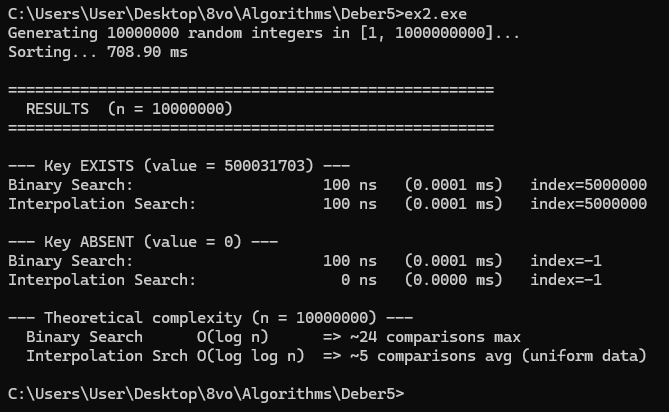
\includegraphics[width=0.9\linewidth]{imagenes/salida2.png}
    \caption{Execution output for Binary vs Interpolation Search on $10^7$ elements}
\end{figure}

As observed, both are remarkably fast (a few hundred nanoseconds). While Interpolation Search theoretically requires fewer steps (5 vs 24), the computational overhead of the division and multiplication per step makes their absolute execution times practically identical on modern CPUs. Notice the absent key case is faster in Interpolation Search because it immediately evaluates bounds and halts.

\newpage
% ================================================================== %
%  EXERCISE 3
% ================================================================== %
\section{Topological Sort Has a Solution If and Only If the Graph Is a DAG}

\subsection{Problem Statement}

\begin{infobox}
\textit{``Prove that the topological sorting problem has a solution
if and only if it is a DAG.''}
\end{infobox}

\subsection{Formal Mathematical Proof}

\begin{theorem}
A directed graph $G = (V, E)$ has a topological ordering \textbf{if and
only if} $G$ is a Directed Acyclic Graph (\DAG).
\end{theorem}

\begin{proof}
Let $G=(V,E)$ be a directed graph.

We need to prove:
\[ G \text{ has a topological ordering } \iff G \text{ is a DAG} \]

% =============================
\paragraph{($\Rightarrow$)\enspace If $G$ has a topological ordering, then $G$ is a DAG.}

Suppose that $G$ has a topological ordering. By definition, for every directed edge $u \to v$, the vertex $u$ must appear before $v$ in the ordering.

Assume that $G$ contains a directed cycle:
\[ v_1 \to v_2 \to \cdots \to v_k \to v_1 \]

The first $k-1$ edges require:
\[ v_1 < v_2 < \cdots < v_k \]
But the last edge $v_k \to v_1$ requires:
\[ v_k < v_1 \]

This is impossible because we cannot have both $v_1 < v_k$ and $v_k < v_1$.
Therefore, $G$ cannot contain a directed cycle. Hence, $G$ is a DAG. \hfill$\checkmark$

% =============================
\paragraph{($\Leftarrow$)\enspace If $G$ is a DAG, then $G$ has a topological ordering.}

Now suppose that $G$ is a DAG.

A DAG must contain at least one vertex with in-degree 0. Otherwise, if every vertex had an incoming edge, following those incoming edges would eventually create a directed cycle, which contradicts the fact that $G$ is acyclic.

Choose a vertex with in-degree 0 and place it first in the ordering. Then remove that vertex and all its outgoing edges.

The remaining graph is still a DAG, because removing vertices and edges cannot create a cycle. We repeat this process until all vertices have been removed.

The resulting sequence is a topological ordering because, for every edge $u \to v$, vertex $u$ is placed before $v$.

Therefore, a DAG always has a topological ordering. \hfill$\checkmark$

\paragraph{Conclusion}
Since both directions have been proven,
\[ \boxed{G \text{ has a topological ordering if and only if } G \text{ is a DAG}} \]
Therefore, the topological sorting problem has a solution exactly when the directed graph is acyclic.
\end{proof}

\subsection{Algorithmic Proof: Kahn's Algorithm}

The inductive proof naturally translates to Kahn's Algorithm, which practically demonstrates the theorem. The code tracks how many vertices are processed. If we process all $V$ vertices, we successfully built the topological sort (it was a DAG). If the queue empties prematurely, we failed to process vertices locked in a cycle.

\begin{lstlisting}[language=C++, caption={Core of Kahn's Algorithm}]
queue<int> q;
// 1. Find all sources (in-degree 0)
for (int v = 0; v < V; v++) 
    if (inDegree[v] == 0) q.push(v);

int processedCount = 0;
while (!q.empty()) {
    int u = q.front(); q.pop();
    processedCount++; // Vertex u is placed in topological order
    
    // 2. Remove outgoing edges. If a neighbour becomes a source, enqueue it.
    for (int w : adj[u]) {
        if (--inDegree[w] == 0) q.push(w);
    }
}

// 3. Cycle Detection
if (processedCount != V) throw runtime_error("Cycle detected. Not a DAG.");
\end{lstlisting}

\subsection{Execution Output}

\begin{figure}[H]
    \centering
    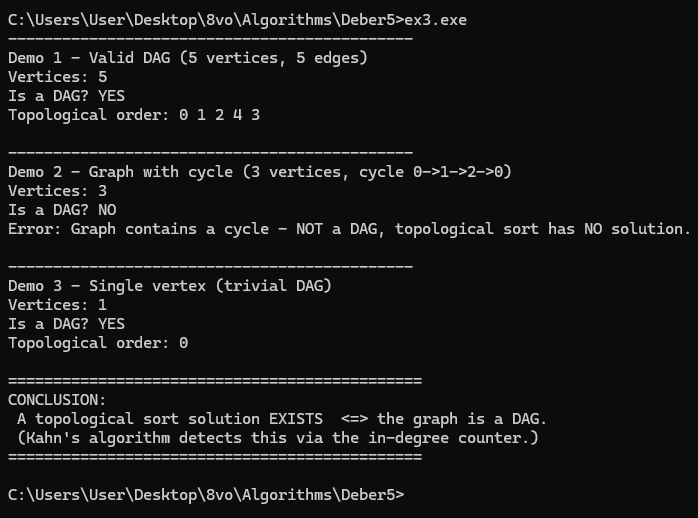
\includegraphics[width=0.9\linewidth]{imagenes/salida3.png}
    \caption{Execution output demonstrating Kahn's algorithm cycle detection}
\end{figure}

\newpage
% ================================================================== %
%  EXERCISE 4
% ================================================================== %
\section{Maximum Distinct Topological Orderings for a DAG with \texorpdfstring{$n$}{n} Vertices}

\subsection{Problem Statement}

\begin{infobox}
\textit{``For a DAG with $n$ vertices, what is the largest number of
distinct solutions the topological sorting problem can have?
Show your solution.''}
\end{infobox}

\subsection{Answer and Mathematical Proof}

\begin{keybox}
\textbf{The maximum number of distinct topological orderings of a
\DAG{} with $n$ vertices is $n!$ (n factorial).}
\end{keybox}

\begin{proof}
Let $G = (V, E)$ be a graph with $n$ vertices. A topological ordering is essentially a permutation of the vertices $V$ that satisfies constraints.

Since there are $n$ distinct vertices, the set of all possible permutations has a cardinality of exactly $n!$. Any topological ordering must belong to this set. Therefore, no graph can possibly have more than $n!$ topological orderings. 

To prove this bound is achievable, consider the \textbf{empty graph} $G_{\emptyset} = (V, \emptyset)$, which has zero edges. Since there are no edges, there are zero dependencies or constraints between vertices. Every vertex constantly has an in-degree of 0. Thus, any of the $n!$ possible permutations of $V$ is valid.

Furthermore, introducing any edge $(u,v)$ to the graph enforces the condition that $u$ must appear before $v$. In exactly half of the $n!$ possible permutations, $u$ precedes $v$, and in the other half, $v$ precedes $u$. Thus, a single edge immediately invalidates half the permutations, reducing the possible topological sorts to $\leq \frac{n!}{2}$. Consequently, the empty graph is the unique structure that maximizes topological orderings.
\end{proof}

\subsection{Algorithmic Verification: DFS Backtracking}

To computationally verify this, we can write a backtracking algorithm that explores all possible valid branches of a topological sort. 

\begin{lstlisting}[language=C++, caption={Backtracking Logic for All Topological Sorts}]
void backtrack() {
    bool found_any_unvisited_source = false;
    for (int v = 0; v < V; v++) {
        // We can pick any unvisited vertex with in-degree 0
        if (!visited[v] && inDegree[v] == 0) {
            found_any_unvisited_source = true;
            visited[v] = true;
            path.push_back(v);
            
            // "Remove" vertex by decrementing neighbours' in-degrees
            for (int w : adj[v]) inDegree[w]--;

            backtrack(); // Recursive exploration

            // Backtrack: Restore state for the next permutation
            for (int w : adj[v]) inDegree[w]++;
            path.pop_back();
            visited[v] = false;
        }
    }
    // If the path length is V, we've found a complete ordering
    if (!found_any_unvisited_source && path.size() == V) {
        results.push_back(path);
    }
}
\end{lstlisting}

This algorithm recursively generates the permutations. Testing the empty graph for sizes $n=1$ to $5$ yields exactly $n!$ results:

\begin{figure}[H]
    \centering
    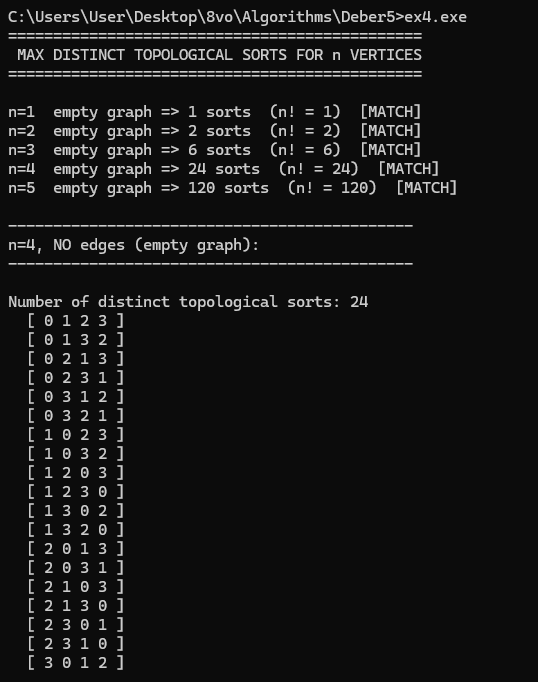
\includegraphics[width=0.85\linewidth]{imagenes/salida4-1.png}
    \\[1em]
    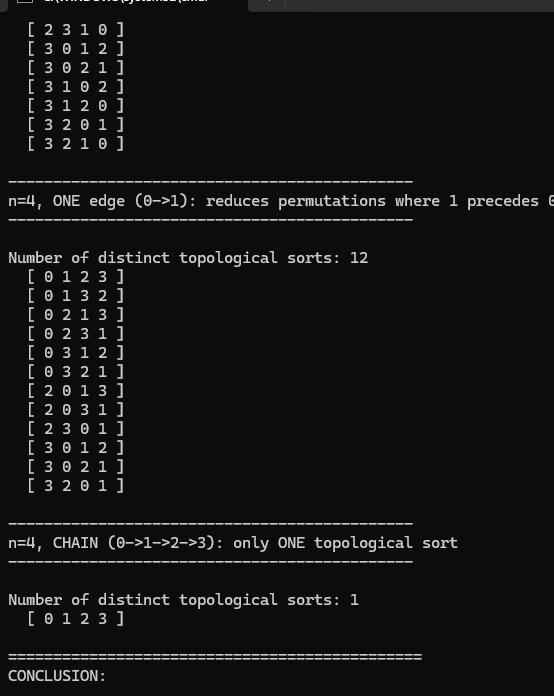
\includegraphics[width=0.85\linewidth]{imagenes/salida4-2.png}
    \caption{Execution output (Part 1): Topological sorts for empty graphs and simple edge}
\end{figure}

\begin{figure}[H]
    \centering
    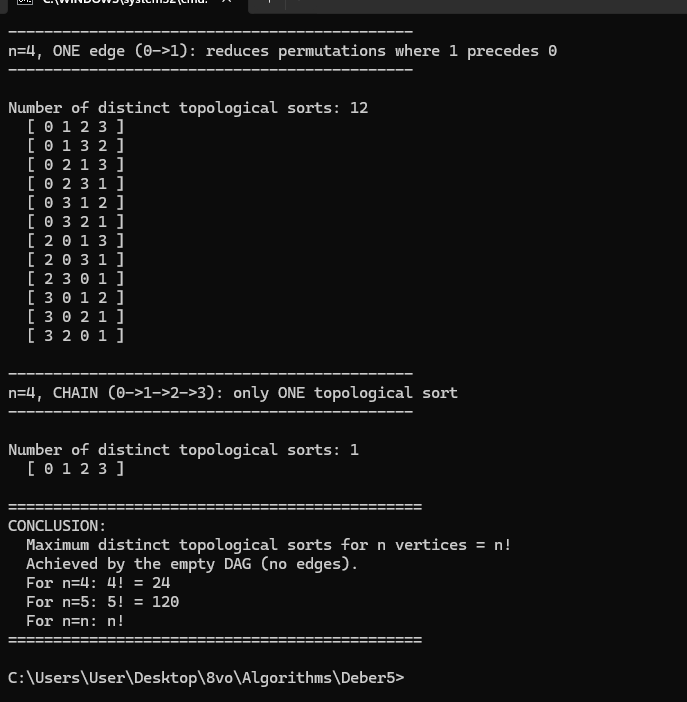
\includegraphics[width=0.85\linewidth]{imagenes/salida4-3.png}
    \caption{Execution output (Part 2): Topological sorts for a chain graph}
\end{figure}

\end{document}
